\chapter{Experiments and Results\label{ExperimentsResults}}

In this section, we introduce the test cases that we intend to use. We
go through the details of our cosine and sum measure scoring schemes
that we will be using to test our systems ability to rank a correct
disease given a list of symptoms. By comparing the individual top
scores of each different measure tested on a given matrix (stemmed or
non-stemmed), we find the most efficient measure to score data on our
system. It should here be noted that each time we score a given
disease, we do it by taking the top 3000\footnote{A number chosen at
  random in between our total number of different diseases} of the
documents returned by the similarity measure and the
\textit{SearchCases} module. Using the most efficient measure, we try
to score 5 blind tests provided by a chief physician.

We provide a description of how clustering could be used to improve
the system, by looking at clusters of diseased ranked far from top
20. We then look at \ldots

\fxnote{Skriv noget her} ... Note: semantic section are still to be written.

Finally, we take discussion on the potential noise of overview
articles and test the potential of consensus normalization.

\section{Test cases}

\subsubsection{BMJ}
In order to test our system we need to find some suitable test cases
that are not biased towards our own system. We have chosen to first of
all test our system against a subset of the disease cases in BMJ
\cite{HangwiTang11102006}, that is disease cases which can be found in
our system\footnote{As mentioned earlier in \ref{Database} our system
  can only help diagnose the diseases contained in the
  system}. However, there is one major difference between the tests
conducted by the people behind the BMJ article - they have a medical
background (a respiratory and sleep physician and a rheumatologists)
contrary to our computer science background. This means that we have
no bias or knowledge about selecting symptoms and --- as they explain ---
given some of the symptoms the correct diagnosis were evident to
them. Note that we will (in the following sections) be referring to
the subset of the test cases as BMJ since this is were it was
found.

The subset of the BMJ test cases include the following 13 diseases (Table \ref{BMJCases}):

\begin{table}[H]
  \caption{Disease / Symptoms list for the 13 BMJ cases}
  \label{BMJCases}
  \begin{scriptsize}
  \begin{tabular}{|l|p{7cm}|}
    \hline
    Disease & Symptoms \\
    \hline
    Infective endocarditis & Acute, aortic,  regurgitation, depression,  abscess \\
    \hline
    Cushing's syndrome & hypertension, adrenal, mass \\
    \hline
    Eosinophilic granuloma & Hip, lesion, older, child \\
    \hline
    Ehrlichiosis & fever, bilateral, thigh, pain, weakness \\
    \hline
    Neurofibromatosis type 1 & multiple, spinal, tumours, skin, tumours \\
    \hline
    Pheochromocytoma & hypertension, papilledema, headache, renal, mass, cafe, au, lait \\
    \hline
    Creutzfeldt-Jakob disease & ataxia, confusion, insomnia, death \\
    \hline
    Churg-Strauss syndrome & Wheeze, weight, loss, ANCA, haemoptysis, haematuria \\
    \hline
    Dermatomyositis & myopathy, neoplasia, dysphagia, rash, periorbital, swelling \\
    \hline
    Cat Scratch Disease & renal, transplant, fever, cat, lymphadenopathy \\
    \hline
    TEN & bullous, skin, conditions, respiratory, failure, carbamazepine \\
    \hline
    MELAS & seizure, confusion, dysphasia, T2, lesions \\
    \hline
    Brugada syndrome & cardiac arrest sleep \\
    \hline
  \end{tabular}
  \end{scriptsize}
\end{table}

\subsubsection{Orpha.net}
To examine significance of the test result, we have additionally
selected some diseases at 'random' from Orpha.net. We require that the
disease has a description on Orpha.net containing a sentence with
'characterized by'. Occasionally we have meant that the 'characterized
by' contained too many specific symptoms (e.g. derivatives of the name
of the disease or a several sentences long list of symptoms) and have
removed certain symptoms from the list. Examples of reductions would
be\footnote{Note that this is based solely on our own judgement as
  non-physicians.}

{\small
\textit{congenital anomalies (microcephaly, specific facial characteristics, broad thumbs and halluces and postnatal growth retardation), intellectual deficit and behavioural characteristics}
}\\

has been reduced to\\

{\small
\textit{congenital anomalies, intellectual deficit, behavioural}
}\\

and\\

{\small
\textit{congenital malformations: hydrocephalus (due to Dandy-Walker anomaly), cleft palate, and severe joint contractures}
}\\

has been reduced to \\

{\small
\textit{congenital malformations: hydrocephalus, cleft palate, severe joint contractures}
}\\

The test cases from Orpha.net include 30 different diseases can be
found in table \ref{OrphanetCases1} and \ref{OrphanetCases2}.

\begin{table}[H]
\caption{Disease / symptom list for 30 Orpha.net test cases}
\label{OrphanetCases1}
\begin{scriptsize}
\begin{tabular}{| p{6cm} | p{6.5cm} |}
\hline
Disease name & Symptom list \\
\hline
Apparent mineralocorticoid excess & early-onset, severe hypertension, associated, low renin levels, hypoaldosteronism \\
\hline
Rubinstein-Taybi syndrome & congenital anomalies, intellectual deficit, behavioural characteristics \\
\hline
Aagenaes syndrome & chronic severe lymphoedema, severe neonatal cholestasis, lessens during early childhood and becomes episodic \\
\hline
Aase Smith syndrome & congenital malformations: hydrocephalus, cleft palate, severe joint contractures \\
\hline
Achondroplasia & short limbs, hyperlordosis, short hands, macrocephaly, high forehead and saddle nose \\
\hline
Acalvaria & missing scalp and flat bones over an area of the cranial vault \\
\hline
Acrodysostosis & abnormally short and malformed bones of the hands and feet (peripheral dysostosis), nasal hypoplasia and mental retardation \\
\hline
Acromegaly & progressive somatic disfigurement (face and extremities) and systemic manifestations \\
\hline
Biliary atresia & biliary obstruction of unknown origin, neonatal period \\
\hline
Bronchiolitis obliterans with obstructive pulmonary disease & inflammatory and fibrosing thickening of bronchiolar walls, airflow obstruction \\
\hline
Cholera & severe diarrhea and vomiting \\
\hline
Choroideremia & progressive degeneration of the choroid, retinal pigment epithelium (RPE), and neural retina \\
\hline
Coats disease & abnormal development of retinal vessels (telangiectasia) with a progressive deposition of intraretinal or subretinal exudates \\
\hline
Omphalocele cleft palate syndrome lethal & omphalocele and cleft palate \\
\hline
Darier disease & keratotic papules in seborrheic areas and specific nail anomalies \\
\hline
Ichthyosis hepatosplenomegaly cerebellar degeneration & ichthyosis, hepatosplenomegaly and late-onset cerebellar ataxia \\
\hline
Emery-Dreifuss muscular dystrophy & muscular weakness and atrophy, with early contractures of the tendons and cardiomyopathy \\
\hline
Costello syndrome & postnatal growth retardation, coarse facies, intellectual deficit, skin anomalies and cardiac abnormalities \\
\hline
Fibrodysplasia ossificans progressiva & congenital malformation of great toes, progressive, disabling heterotopic osteogenesis in predictable anatomical patterns \\
\hline
Acropectorovertebral dysplasia & fusion of the carpal and tarsal bones, with complex anomalies of the fingers and toes \\
\hline
Osteogenesis imperfecta & increased bone fragility and low bone mass \\
\hline
Primary biliary cirrhosis & injury of the intrahepatic bile ducts \\
\hline
Hennekam syndrome & lymphoedema, intestinal lymphangiectasia, intellectual deficit and facial dysmorphism \\
\hline
Hyperlysinemia & elevated levels of lysine in the cerebrospinal fluid and blood \\
\hline
Jackson-Weiss syndrome & tarsal and/or metatarsal coalitions and variable craniosynostosis, accompanied by facial anomalies, broad halluces and normal hands \\
\hline
Jalili syndrome & amelogenesis imperfecta and cone-rod retinal dystrophy \\
\hline
Jeune syndrome & narrow thorax and short limbs \\
\hline
Multiple myeloma & overproduction of abnormal plasma cells in the bone marrow and manifested by skeletal destruction, bone pain, and presence of abnormous immunoglobulins \\
\hline
Trichodental syndrome & fine, dry and short hair with dental anomalies \\
\hline
\end{tabular}
\end{scriptsize}
\end{table}

\subsubsection{Blind tests}
In addition to the BMJ and Orpha.net test cases, we have performed a
blind test on disease cases given by Henrik Jørgensen \cite{TheDude}. 
Here, we were given 5 different test cases and the queries made are 
based on symptoms extracted from the cases based on our own judgement.
The test is done with the highest performing measure and matrix - determined
by the tests run on the BMJ and Orpha.net test cases in section 
\ref{TestingCosineSimilarity}. The results of the blind test can be found
in section \ref{Blindtest}.

\begin{table}[H]
\label{blind_test_table}
\caption{Disease / Give case / Used query for the 5 blind test cases}
\begin{scriptsize}
\label{OrphanetCases1}
\begin{tabular}{| p{3cm} | p{4.5cm} | p{4.5cm} |}
\hline
Disease name & Given case & Used symptom query \\
\hline
Fibrodysplasia ossificans progressiva & Dreng, normal ved f\o dslen bortset fra deformitet af begge storeter (de manglede et led). Udvikler sig normalt efterfl\o gende. Ved 5 \aa rs alderen der viser knoglev\ae v uden malignitetstegn. Kort tid efter biopsien udvikles mere knoglev\ae kst, pr\ae cis der hvor man har sk\ae ret. & Boy, normal birth, deformity of both big toes (missing joint), quick development of bone tumor near spine and osteogenesis at biopsy.\\
\hline
Adrenoleukodystrophy autosomal neonatal form & Normally developed boy until age 5, where he progressively developed the following symptoms: Talking difficulties, seizures, ataxia, adrenal insufficiency and  degeneration of visual and auditory functions.& Normally developed boy age 5, progessive development of talking difficulties, seizures, ataxia, adrenal insufficiency and  degeneration of visual and auditory functions \\
\hline
Papillon Lefevre syndrome & A boy age 14 comes to the doctor with yellow, keratotic plaques on the skin of his palms and soles going up onto the dorsal side. Both hands and feet are affected. He equally had swollen and very vulnerable gums since the age of 4 with loss of most of his permanent teeth. & Boy age 14, yellow, keratotic plaques on the skin of palms and soles going up onto the dorsal side. Both hands and feet are affected.\\
\hline
Kleine Levin Syndrome & 16-\aa rig j\o disk dreng har en til to gange om maaneden anfald, hvor han f\o rst og fremmest skal sove utroligt meget - ca. 18 timer om dagen. Anfaldene varer ca en uges tid. Han \ae ndrer karakter under anfaldene og bliver irritabel og aggressiv, n\aa r han v\ae kkes. N\aa r han er v\aa gen i anfaldsperioden spiser han helt utroligt store m\ae ngder mad, og hans appetit p\aa sex er endvidere abnormt stor. & Jewish boy age 16, monthly seizures, sleep deficiency, aggressive and irritable when woken, highly increased sexual appetite and hunger.\\
\hline
Schinzel-Giedion Syndrome & The patient is a male child presenting at birth with numerous malformations. He had midfacial retraction with a deep groove under the eyes, and hypertelorism. A short nose with a low nasal bridge and large low-set ears were noted. He had a wide mouth and retrognathia. Hypertrichosis with bright reddish hair and a median frontal cutaneous angioma were present. The neck was short with redundant skin. Bilateral inguinal hernias, hypospadias with a megameatus, and cryptorchidism were noted. & Male child, malformations at birth, midfacial retraction with a deep groove under the eyes, and hypertelorism, short nose with a low nasal bridge and large low-set ears, wide mouth and retrognathia. Hypertrichosis with bright reddish hair and a median frontal cutaneous angioma, short neck with redundant skin, Bilateral inguinal hernias, hypospadias with a megameatus, and cryptorchidism \\
\hline
\end{tabular}
\end{scriptsize}
\end{table}

\subsection{Scoring schemes}

As mentioned in the previous chapters, we will employ two different
kinds of scoring measures - the cosine and sum measure. The original
idea --- behind using a sum measure --- was to test how much the cosine
measure would outperform this simpler measure but as we shall see in
section \ref{TestingCosineSimilarity} and section
\ref{TestingSumSimilarity}, the cosine measure is actually
outperformed itself by the sum measure. We will try to explain this
'oddity' in the given section and for now focus the way we use the two
different kinds of measure. The following cosine and sum score
measures are described in accordance to how they function on the term
document matrix. The exception of the disease matrix is described at
the end of this section.

\subsubsection{The cosine score\label{CosineScore}}

We will be testing the following three different approaches to using
the cosine similarity measure: cosine mean, cosine median and cosine
max.

\subsubsection{Cosine mean}
Every disease has one or more documents attached to it (as described
in section \ref{Database}). This means that the same disease might be
returned many times when looking at a top score of document similarity
measures produced by for example the cosine score. Therefore --- to
give each disease a score --- we use a form of consensus method where
we sum the scores of each document belonging to that disease. This
produces a mean score of each disease.

When the system (or more specifically the Query module) receives a
query, it ranks the query vector of terms against all document vectors
in which one or more of the terms has appeared. This results in a list
of scores $\mathbf{x}_{\textrm{all diseases}} = \left\{x_1, x_2,
\dots, x_n \right\}$. It then runs through every scored document and
adds the score to the disease from which the document came (in
accordance to the consensus method just described). Since some
documents appear in more than one disease (see section
\ref{Database}), several diseases might have the sum of a single
document added to its score $\mathbf{x}_{\textrm{disease}_{1}} =
\left\{x_{\textrm{sum for} x_2, x_7, x_i, \dots, x_j}\right\}$,
$\mathbf{x}_{\textrm{disease}_{2}} = \left\{x_{\textrm{sum for} x_1,
  x_2, x_9, \dots, x_47, x_n}\right\}, \dots$. Lastly, we evaluate the
total ranking of each disease. We combine each
$x_{\textrm{disease}_1}$, $x_{\textrm{disease}_2}$ into a list of all
the returned disease scores $\mathbf{\mathit{SL}} =
\left\{x_{\textrm{disease}_1},x_{\textrm{disease}_2}, \dots,
x_{\textrm{disease}_n}\right\}$. These are then sorted and the highest
scoring is deemed the most likely to be the correct disease given the
query vector.

\subsubsection{Cosine median}
The median is calculated much like the mean, except for selecting the
median of $\mathbf{x}_{\textrm{disease}_{1}} = \left\{x_2,x_7, x_i,
\dots, x_j\right\}, \mathbf{x}_{\textrm{disease}_{2}}, \dots,
\mathbf{x}_{\textrm{disease}_{n}}$, instead of summing the scores as
we did above.

\subsubsection{Cosine max}
Does the same as above, except that it selects the maximum scoring in each
disease lists and sort the resulting list and select the highest
scoring as the most probable.

\subsubsection{The sum score}

The sum measure works exactly like the cosine mean measure, except for
running on non-normalized vectors. See \ref{VectorSimilarity} for
reasoning.

\subsubsection{The disease matrix exception}

This is a short description on how we use the cosine and sum measures
on the disease matrix. The disease matrix has no document vectors and
is solely made up of summed disease vectors. This means that there is
no point in using cosine mean, median or max, as there is no multiple
label occurrences to run a consensus method over. Here the score is
either the cosine or sum measure calculated for each of the diseases
that contain the queried term(s).

\subsection{Testing the cosine similarity measure\label{TestingCosineSimilarity}}

The first test we run is on for the three different cosine scoring
measures - mean, median and max. On the two bar charts below
\ref{termDoc_bmj_hist_3000_ns_mea_med_max_nc} and
\ref{termDoc_orphan_hist_3000_ns_mea_med_max_nc} the query scores of
the BMJ and the Orhpa.net test cases are shown. These are run on the
non-stemmed term document matrix. The scores a drawn on a logarithmic
scale while the 'real' scores a shown below each chart. Note that the
values are 0-indexed(!) and all tests are performed on TF-IDF
preprocessed matrices.

\begin{figure}[H]
  \caption{Test for mean, median and max cosine measure on a non-stemmed term-doc}
  \begin{center}
    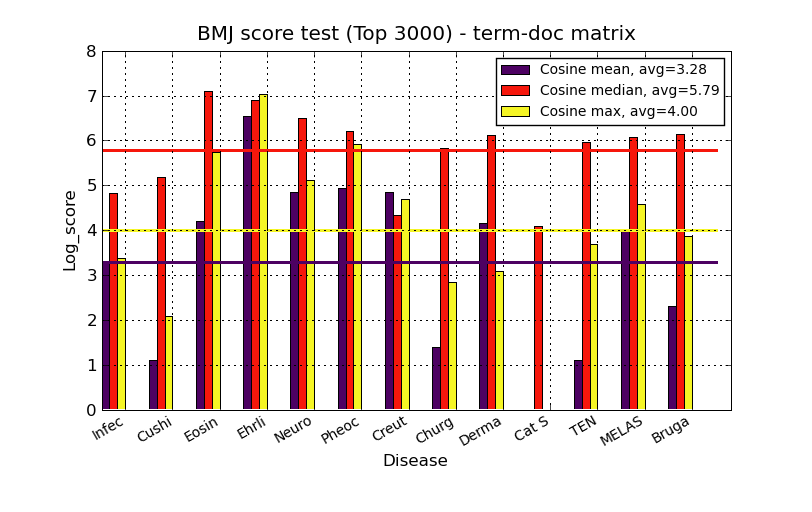
\includegraphics[width=1.2\textwidth]{barcharts/termDoc_bmj_hist_3000_ns_mea_med_max_nc.png}
  \end{center}
  \label{termDoc_bmj_hist_3000_ns_mea_med_max_nc}
\end{figure}

\begin{table}[H]
  \begin{tiny}
  \label{testResult_termDoc_bmj_hist_3000_ns_mea_med_max_nc}
  \begin{tabular}{|l|r|r|r|r|r|r|r|}
    \hline
    Measure &Infec&Cushi&Eosin&Ehrli&Neuro&Pheoc&Creut \\
    \hline
    Cosine: mean & 25 & 2 & 66 & 692 & 128 & 139 & 128 \\
    \hline
    Cosine: median & 123 & 179 & 1210 & 1004 & 665 & 502 & 76 \\
    \hline
    Cosine: max & 28 & 7 & 311 & 1123 & 166 & 375 & 109  \\
    \hline
  \multicolumn{8}{c}{} \\
  \end{tabular}
  \begin{tabular}{|l|r|r|r|r|r|r|r|}
    \hline
    Measure &Churg&Derma&Cat S&TEN&MELAS&Bruga& \scriptsize{\textbf{\# in top 20}} \\
    \hline
    Cosine: mean non-stemmed & 3 & 63 & 0 & 2 & 52 & 9 & \scriptsize{\textbf{5}} \\
    \hline
    Cosine: mean stemmed & 343 & 455 & 59 & 392 & 430 & 464 &  \scriptsize{\textbf{0}}\\
    \hline
    Cosine: max non-stemmed & 16 & 21 & 0 & 39 & 96 & 47 & \scriptsize{\textbf{3}} \\
    \hline
  \end{tabular}
  \end{tiny}
\end{table}

\begin{figure}[H]
  \caption{Test of mean, median and max cosine measure on a non-stemmed term-doc}
  \begin{center}
    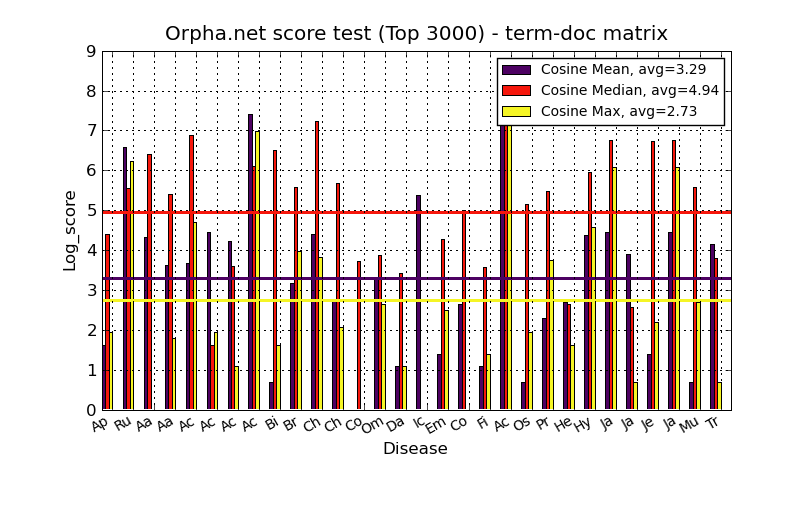
\includegraphics[width=1.2\textwidth]{barcharts/termDoc_orphan_hist_3000_ns_mea_med_max_nc.png}
  \end{center}
  \label{termDoc_orphan_hist_3000_ns_mea_med_max_nc}
\end{figure}

\begin{table}[H]
  \label{testResult_termDoc_orphan_hist_3000_ns_mea_med_max_nc}
  \begin{tiny}
    \begin{tabular}{|l|r|r|r|r|r|r|r|r|r|r|r|r|r|r|r|r|r|r|r|r|r|r|r|r|r|r|r|r|r|r|r|}
      \hline
      Measure &Ap&Ru&Aa&Aa&Ac&Ac&Ac&Ac&Bi&Br&Ch&Ch&Co&Om&Da\\
      \hline
      Cosine: mean & 4 & 664 & 30 & 47 & 38 & 85 & 62 & 1371 & 1 & 32 & 83 & 15 & 0 & 26 & 2 \\
      \hline
      Cosine: median & 163 & 357 & 76 & 240 & 948 & 4 & 76 & 141 & 384 & 314 & 505 & 211 & 44 & 181 & 42 \\
      \hline
      Cosine: max & 4 & 858 & 0 & 10 & 44 & 15 & 2 & 541 & 4 & 116 & 99 & 18 & 0 & 6 & 2\\
      \hline
      \multicolumn{16}{c}{} \\
    \end{tabular}
    \begin{tabular}{|l|r|r|r|r|r|r|r|r|r|r|r|r|r|r|r|r|r|r|r|r|r|r|r|r|r|r|r|r|r|r|}
      \hline
      Measure &Ic&Em&Co&Fi&Ac&Os&Pr&He&Hy&Ja&Ja&Je&Ja&Mu&Tr &  \scriptsize{\textbf{\# in top 20}} \\
      \hline
      Cosine: mean & 81 & 3 & 16 & 2 & 3000 & 4 & 10 & 13 & 24 & 66 & 35 & 3 & 66 & 4 & 34 & \scriptsize{\textbf{13}} \\
      \hline
      Cosine: median & 773 & 87 & 169 & 189 & 3000 & 179 & 265 & 21 & 491 & 692 & 37 & 435 & 692 & 358 & 233 & \scriptsize{\textbf{1}} \\
      \hline
      Cosine: max  & 0 & 22 & 0 & 3 & 3000 & 9 & 67 & 5 & 63 & 201 & 1 & 8 & 201 & 9 & 0 & \scriptsize{\textbf{19}} \\
      \hline
    \end{tabular}
  \end{tiny}
\end{table}

As we see here, the mean cosine measure performs best in the BMJ test
set while the max cosine measure scores best in the Orpha.net test
set. The median measure has an overall low score and running some
quick tests on the different matrices, quickly reveals that median is
not well suited as a measure to take into consideration. Therefore we
will not be testing further on the cosine median score and continues
with the two remaining scores from here on. Note that the score that
has the worst performance in the Orpha.net test. It can and will
happen that diseases are not found within the top 3000 documents that
is returned. When this is the case --- to avoid confusion in the bar
charts and statistics --- we simply set the score of any disease not
found to the value 3000, representing a bad performance. Note also
that a missing bar represents the top score 0.

We now continue testing the scoring measures, this time comparing the
non-stemmed and stemmed term document matrices. The results are shown
in the figures \ref{termDoc_bmj_hist_3000_ns_mea_s_mea_ns_max_s_max}
and \ref{termDoc_orphan_hist_3000_ns_mea_s_mea_ns_max_s_max} below.

\begin{figure}[H]
  \caption{Comparison of mean and max cosine measure tests on non-stemmed and stemmed term-doc matrices}
  \begin{center}
    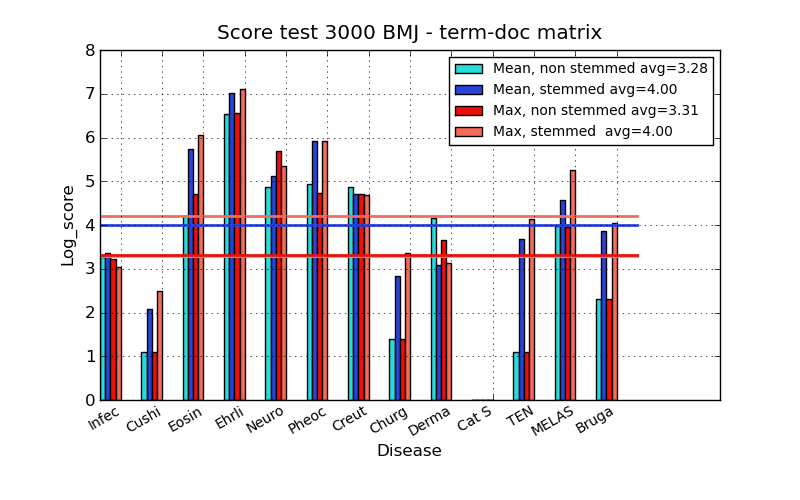
\includegraphics[width=1.2\textwidth]{barcharts/termDoc_bmj_hist_3000_ns_mea_s_mea_ns_max_s_max.png}
  \end{center}
  \label{termDoc_bmj_hist_3000_ns_mea_s_mea_ns_max_s_max}
\end{figure}

\begin{table}[H]
  \begin{tiny}
  \label{testResult_termDoc_bmj_hist_3000_ns_mea_s_mea_ns_max_s_max}
  \begin{tabular}{|l|r|r|r|r|r|r|r|}
    \hline
    Measure &Infec&Cushi&Eosin&Ehrli&Neuro&Pheoc&Creut \\
    \hline
    Cosine: mean non-stemmed &25&2&66&692&128&139&128 \\
    \hline
    Cosine: mean stemmed &24&2&110&710&292&113&110 \\
    \hline
    Cosine: max non-stemmed &28&7&311&1123&166&375&109 \\
    \hline
    Cosine: max stemmed &20&11&427&1232&210&370&108 \\
    \hline
  \multicolumn{8}{c}{} \\
  \end{tabular}
  \begin{tabular}{|l|r|r|r|r|r|r|r|}
    \hline
    Measure &Churg&Derma&Cat S&TEN&MELAS&Bruga& \scriptsize{\textbf{\# in top 20}} \\
    \hline
    Cosine: mean non-stemmed &3&63&0&2&52&9& \scriptsize{\textbf{5}} \\
    \hline
    Cosine: mean stemmed &3&38&0&2&51&9& \scriptsize{\textbf{5}}\\
    \hline
    Cosine: max non-stemmed &16&21&0&39&96&47& \scriptsize{\textbf{3}} \\
    \hline
    Cosine: max stemmed &28&22&0&62&192&56& \scriptsize{\textbf{2}} \\
    \hline
  \end{tabular}
  \end{tiny}
\end{table}

\begin{figure}[H]
  \caption{Comparison of mean and max cosine measure tests on non-stemmed and stemmed term-doc matrices}
  \begin{center}
    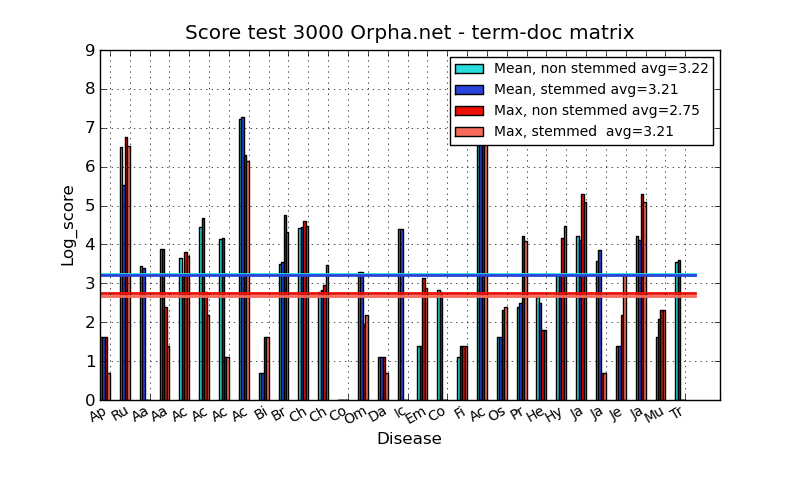
\includegraphics[width=1.2\textwidth]{barcharts/termDoc_orphan_hist_3000_ns_mea_s_mea_ns_max_s_max.png}
  \end{center}
  \label{termDoc_orphan_hist_3000_ns_mea_s_mea_ns_max_s_max}
\end{figure}

\begin{table}[H]
\label{testResult_termDoc_orphan_hist_3000_ns_mea_s_mea_ns_max_s_max}
\begin{tiny}
  \begin{tabular}{|l|r|r|r|r|r|r|r|r|r|r|r|r|r|r|r|r|r|r|r|r|r|r|r|r|r|r|r|r|r|r|r|}
    \hline
    Measure &Ap&Ru&Aa&Aa&Ac&Ac&Ac&Ac&Bi&Br&Ch&Ch&Co&Om&Da\\
    \hline
    Cosine: mean non-stemmed &4&664&30&47&38&85&62&1371&1&32&83&15&0&26&2\\
    \hline
    Cosine: mean stemmed &4&248&29&48&23&106&64&1436&1&34&85&16&0&26&2\\
    \hline
    Cosine: max non-stemmed &4&858&0&10&44&15&2&541&4&116&99&18&0&6&2\\
    \hline
    Cosine: max stemmed &1&677&0&3&40&8&2&462&4&75&87&31&0&8&1 \\
    \hline
    \multicolumn{16}{c}{} \\
    \end{tabular}
    \begin{tabular}{|l|r|r|r|r|r|r|r|r|r|r|r|r|r|r|r|r|r|r|r|r|r|r|r|r|r|r|r|r|r|r|}
    \hline
     Measure &Ic&Em&Co&Fi&Ac&Os&Pr&He&Hy&Ja&Ja&Je&Ja&Mu&Tr &\scriptsize{\textbf{\# in top 20}} \\
    \hline
    Cosine: mean non-stemmed  &81&3&16&2&3000&4&10&13&24&66&35&3&66&4&34 & \scriptsize{\textbf{13}} \\
    \hline
    Cosine: mean stemmed &81&3&15&3&3000&4&11&11&24&60&46&3&60&7&36 & \scriptsize{\textbf{13}} \\
    \hline
    Cosine: max non-stemmed &81&3&15&3&3000&4&11&11&24&60&46&3&60&7&36 & \scriptsize{\textbf{19}} \\
    \hline
    Cosine: max stemmed &0&22&0&3&3000&9&67&5&63&201&1&8&201&9&0 & \scriptsize{\textbf{18}} \\
    \hline
  \end{tabular}
\end{tiny}
\end{table}

The two score tests just performed now presents us with a dilemma. In the BMJ test set 
the 'mean stemmed' and 'non-stemmed' scores performs best while in the Orpha.net test set, 
it is just the opposite. We have chosen to cope with this by taking out the top score 
measure for each of the test sets - 'mean non-stemmed' from BMJ and 'max stemmed' from 
the Orpha.net.

The next step is to analyse our data by performing a square root transformation 
\ref{SquareRoot} of the TF-IDF preprocessed data above. Note that it is required that 
all values transformed are between 0 and 1 which in our case is secured by the fact 
that the matrices, we use for the cosine measure, are normalized. The reason for the 
square root analysis is that it allows us to see whether the data has been correctly 
weighted. The square root transformation raises small values by a greater degree than 
it does large values. This means that if our scores improve, the information containing 
terms in the term document matrix have not been given high enough values by the applied 
heuristics.

The tests are shown in the figures below, where we compare the best measures from above 
with their square root transformation.

\begin{figure}[H]
  \caption{Comparison of mean (non-stemmed term-doc) and max (stemmed term-doc) cosine measure tests with and without sqrt-transformation}
  \begin{center}
    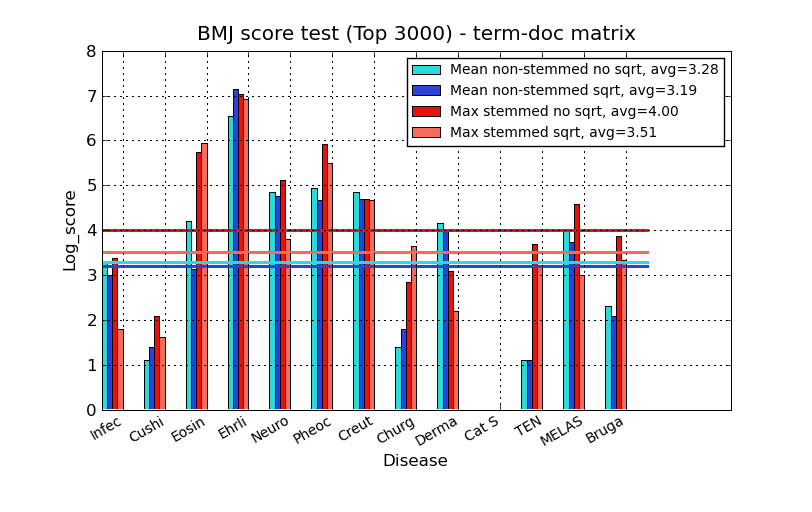
\includegraphics[width=1.2\textwidth]{barcharts/termDoc_bmj_hist_3000_ns_mea_ns_mea_sqr_s_max_s_max_sqr.png}
  \end{center}
  \label{termDoc_bmj_hist_3000_ns_mea_ns_mea_sqr_s_max_s_max_sqr}
\end{figure}

\begin{table}[H]
  \label{testResult_termDoc_bmj_hist_3000_ns_mea_ns_mea_sqr_s_max_s_max_sqr}
  \begin{tiny}
    \begin{tabular}{|l|r|r|r|r|r|r|r|}
      \hline
      Measure &Infec&Cushi&Eosin&Ehrli&Neuro&Pheoc&Creut \\
      \hline
      Cosine: mean non-stemmed no sqrt &25&2&66&692&128&139&128 \\
      \hline
      Cosine: mean non-stemmed sqrt &19&3&22&1268&115&105&108 \\
      \hline
      Cosine: max stemmed no sqrt &20&11&427&1232&210&370&108 \\
      \hline
      Cosine: max stemmed sqrt &2&10&136&1123&68&249&130 \\
      \hline
      \multicolumn{8}{c}{} \\
    \end{tabular}
    \begin{tabular}{|l|r|r|r|r|r|r|r|}
      \hline
      Measure &Churg&Derma&Cat S&TEN&MELAS&Bruga& \scriptsize{\textbf{\# in top 20}} \\
      \hline
      Cosine: mean non-stemmed no sqrt &3&63&0&2&52&9 &\scriptsize{\textbf{5}} \\
      \hline
      Cosine: mean non-stemmed sqrt &5&54&0&2&41&7 &\scriptsize{\textbf{6}}\\
      \hline
      Cosine: max stemmed no sqrt &28&22&0&62&192&56 & \scriptsize{\textbf{2}} \\
      \hline
      Cosine: max stemmed sqrt &44&8&0&47&65&25 & \scriptsize{\textbf{4}} \\
      \hline
    \end{tabular}
  \end{tiny}
\end{table}

\begin{figure}[H]
  \caption{Comparison of mean (non-stemmed term-doc) and max (stemmed term-doc) cosine measure tests with and without sqrt-transformation}
  \begin{center}
    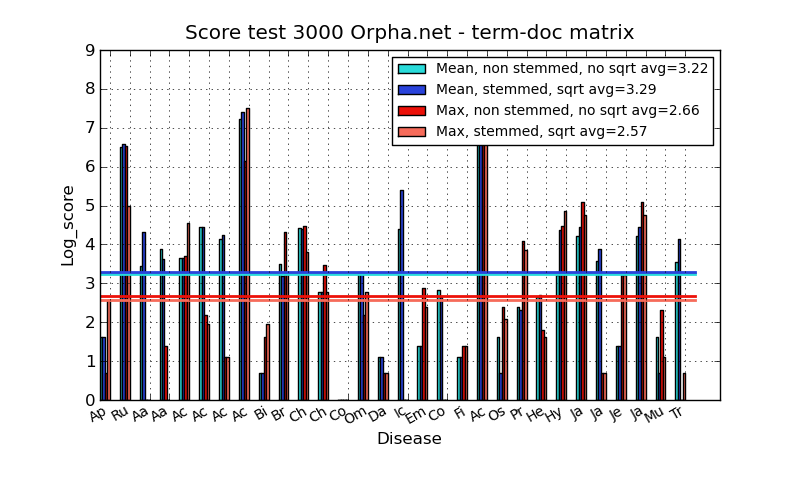
\includegraphics[width=1.2\textwidth]{barcharts/termDoc_orphan_hist_3000_ns_mea_ns_mea_sqr_s_max_s_max_sqr.png}
  \end{center}  
  \label{termDoc_orphan_hist_3000_ns_mea_ns_mea_sqr_s_max_s_max_sqr}
\end{figure}

\begin{table}[H]
\label{testResult_termDoc_orphan_hist_3000_ns_mea_ns_mea_sqr_s_max_s_max_sqr}
\begin{tiny}
  \begin{tabular}{|l|r|r|r|r|r|r|r|r|r|r|r|r|r|r|r|r|r|r|r|r|r|r|r|r|r|r|r|r|r|r|r|}
    \hline
    Measure &Ap&Ru&Aa&Aa&Ac&Ac&Ac&Ac&Bi&Br&Ch&Ch&Co&Om&Da\\
    \hline
    Cosine: mean non-stemmed no-sqrt &4&664&30&47&38&85&62&1371&1&32&83&15&0&26&2\\
    \hline
    Cosine: mean non-stemmed sqrt &4&725&75&37&38&85&68&1651&1&23&80&15&0&26&2\\
    \hline
    Cosine: max stemmed no-sqrt &1&677&0&3&40&8&2&462&4&75&87&31&0&8&1\\
    \hline
    Cosine: max stemmed sqrt &12&145&0&0&93&6&2&1842&6&25&44&15&0&15&1 \\
    \hline
    \multicolumn{16}{c}{} \\
    \end{tabular}
    \begin{tabular}{|l|r|r|r|r|r|r|r|r|r|r|r|r|r|r|r|r|r|r|r|r|r|r|r|r|r|r|r|r|r|r|}
    \hline
     Measure &Ic&Em&Co&Fi&Ac&Os&Pr&He&Hy&Ja&Ja&Je&Ja&Mu&Tr &\scriptsize{\textbf{\# in top 20}} \\
    \hline
    Cosine: mean non-stemmed no-sqrt &81&3&16&2&3000&4&10&13&24&66&35&3&66&4&34 & \scriptsize{\textbf{13}} \\
    \hline
    Cosine: mean non-stemmed sqrt &218&3&13&2&3000&1&9&14&78&84&48&3&84&1&62 & \scriptsize{\textbf{13}} \\
    \hline
    Cosine: max stemmed no sqrt &0&17&0&3&3000&10&58&5&86&162&1&24&162&9&0 & \scriptsize{\textbf{18}} \\
    \hline
    Cosine: max stemmed sqrt &0&10&0&3&3000&7&46&4&128&115&1&24&115&2&1 & \scriptsize{\textbf{19}} \\
    \hline
  \end{tabular}
\end{tiny}
\end{table}

These tests reveal some interesting results. Looking at the BMJ test set we see an overall 
improvement in the performance of the square root transformed measures. In Orpha.net test 
set there is an improvement in 'max stemmed' measure while a slight worsening of the 'mean 
non-stemmed' measure. However, there is no change in the number of top 20 results and the 
other measures shows a more significant improvement than the worsening of the last mentioned 
measure. Based on these results, we will not deny that the data in the TF-IDF matrices are 
not as optimized as could have been expected. But we can not say if these anomalies stem from 
the data or the calculations themselves. For now, we choose to view the square root 
transformation as a general improvement.

In section \ref{DiseaseMatrix}, we will be using the best measure of the cosine scoring tests 
executed above - the 'mean stemmed sqrt' and the 'max stemmed sqrt' cosine similarity measures.

\subsection{Testing the sum similarity measure\label{TestingSumSimilarity}}

In this section, we perform the same tests as described in the
previous section, except for the square root transformation which
makes no sense since we will be running on unnormalized data. Or in
other word on values above and below 1 (see section
\ref{SquareRoot}). The first test is run for the mean, median and max
sum measures on a TF-IDF non-normalized term document matrix. The
results are shown on the figures
\ref{termDoc_bmj_hist_3000_sum_mea_med_max} below.

\begin{figure}[H]
  \caption{Test of mean, median and max sum measure on a non-stemmed term-doc matrix}
  \begin{center}
    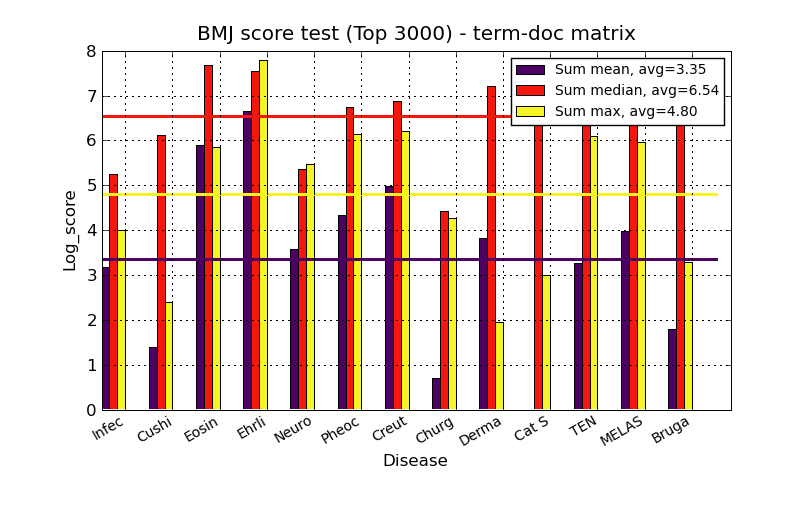
\includegraphics[width=1.2\textwidth]{barcharts/termDoc_bmj_hist_3000_sum_mea_med_max.png}
  \end{center}
  \label{termDoc_bmj_hist_3000_sum_mea_med_max}
\end{figure}

\begin{table}[H]
  \begin{tiny}
    \label{testResult_termDoc_bmj_hist_3000_sum_mea_med_max}
    \begin{tabular}{|l|r|r|r|r|r|r|r|}
      \hline
      Measure &Infec&Cushi&Eosin&Ehrli&Neuro&Pheoc&Creut \\
      \hline
      Sum: mean &23&3&362&772&35&76&144 \\
      \hline
      Sum: median &188&459&2150&1878&213&852&974 \\
      \hline
      Sum: max &54&10&344&2401&235&469&495  \\
      \hline
      \multicolumn{8}{c}{} \\
    \end{tabular}
    \begin{tabular}{|l|r|r|r|r|r|r|r|}
      \hline
      Measure &Churg&Derma&Cat S&TEN&MELAS&Bruga& \scriptsize{\textbf{\# in top 20}} \\
      \hline
      Sum: mean non-stemmed &1&45&0&25&53&5& \scriptsize{\textbf{4}} \\
      \hline
      Sum: mean stemmed &83&1353&670&2193&689&1210 &  \scriptsize{\textbf{0}}\\
      \hline
      Sum: max non-stemmed &70&6&19&441&391&26 & \scriptsize{\textbf{3}} \\
      \hline
    \end{tabular}
  \end{tiny}
\end{table}

\begin{figure}[H]
  \caption{Test of mean, median and max sum measure on a non-stemmed term-doc matrix}
  \begin{center}
    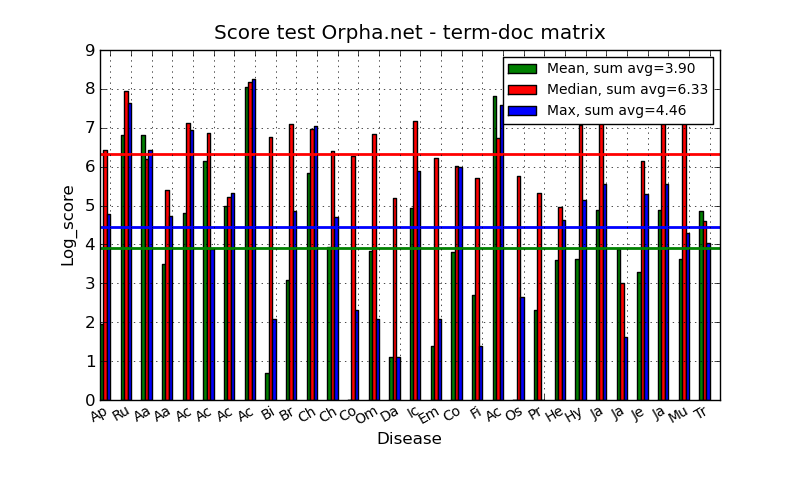
\includegraphics[width=1.2\textwidth]{barcharts/termDoc_orphan_hist_3000_ns_mea_med_max_sum.png}
  \end{center}
  \label{termDoc_orphan_hist_3000_ns_mea_med_max_sum}
\end{figure}

\begin{table}[H]
  \label{testResult_termDoc_orphan_hist_3000_ns_mea_med_max_sum}
  \begin{tiny}
    \begin{tabular}{|l|r|r|r|r|r|r|r|r|r|r|r|r|r|r|r|r|r|r|r|r|r|r|r|r|r|r|r|r|r|r|r|}
      \hline
      Measure &Ap&Ru&Aa&Aa&Ac&Ac&Ac&Ac&Bi&Br&Ch&Ch&Co&Om&Da\\
      \hline
      Sum: mean &6&910&917&32&122&460&145&3119&1&21&342&50&0&45&2 \\
      \hline
      Sum: median &626&2814&495&219&1232&963&182&3590&872&1207&1056&595&526&940&179 \\
      \hline
      Sum: max &119&2081&611&113&1031&48&203&3833&7&127&1139&109&9&7&2\\
      \hline
      \multicolumn{16}{c}{} \\
    \end{tabular}
    \begin{tabular}{|l|r|r|r|r|r|r|r|r|r|r|r|r|r|r|r|r|r|r|r|r|r|r|r|r|r|r|r|r|r|r|}
      \hline
      Measure &Ic&Em&Co&Fi&Ac&Os&Pr&He&Hy&Ja&Ja&Je&Ja&Mu&Tr &  \scriptsize{\textbf{\# in top 20}} \\
      \hline
      Sum: mean &137&3&44&14&2458&0&9&36&37&132&47&26&132&37&127 & \scriptsize{\textbf{8}} \\
      \hline
      Sum: median &1292&503&408&304&845&320&204&143&1165&1763&19&467&1763&1532&100& \scriptsize{\textbf{1}} \\
      \hline
      Sum: max  &357&7&401&3&1957&13&0&102&169&260&4&198&260&72&55 & \scriptsize{\textbf{9}} \\
      \hline
    \end{tabular}
  \end{tiny}
\end{table}

Like in the previous section, we again see the poor results given by the median measure and discards 
this for further testing. In the next tests, we compare the mean and sum measure in the stemmed and 
non-stemmed matrices. The tests are shown on the figures \ref{termDoc_bmj_hist_3000_ns_s_mea_max_sum} 
and \ref{termDoc_orphan_hist_3000_ns_s_mea_max_sum}.

\begin{figure}[H]
  \caption{Comparison of mean and max sum measure tests on non-stemmed and stemmed term-doc matrices}
  \begin{center}
    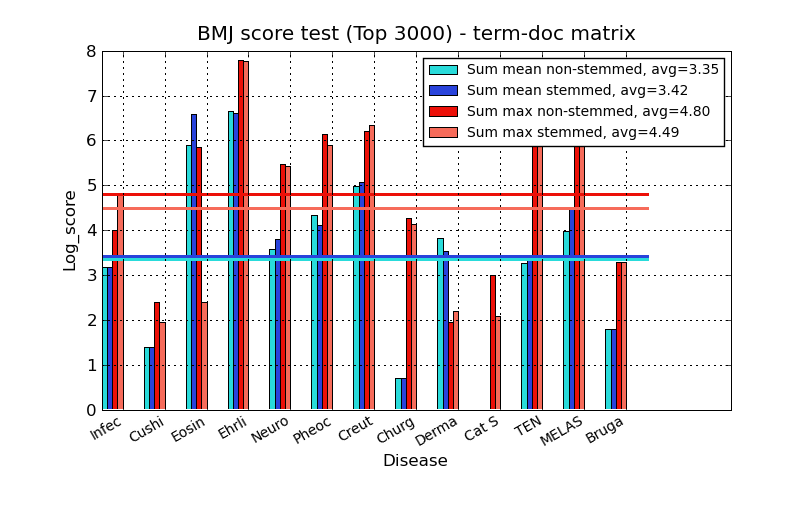
\includegraphics[width=1.2\textwidth]{barcharts/termDoc_bmj_hist_3000_ns_s_mea_max_sum.png}
  \end{center}
  \label{termDoc_bmj_hist_3000_ns_s_mea_max_sum}
\end{figure} 

\begin{table}[H]
  \begin{tiny}
    \label{testResult_termDoc_bmj_hist_3000_ns_s_mea_max_sum}
    \begin{tabular}{|l|r|r|r|r|r|r|r|}
      \hline
      Measure &Infec&Cushi&Eosin&Ehrli&Neuro&Pheoc&Creut \\
      \hline
      Sum: mean non-stemmed &23&3&362&772&35&76&144 \\
      \hline
      Sum: mean stemmed &23&3&720&746&44&60&158 \\
      \hline
      Sum: max non-stemmed &54&10&344&2401&235&469&495 \\
      \hline
      Sum: max stemmed &120&6&10&2374&228&360&566 \\
      \hline
      \multicolumn{8}{c}{} \\
    \end{tabular}
    \begin{tabular}{|l|r|r|r|r|r|r|r|}
      \hline
      Measure &Churg&Derma&Cat S&TEN&MELAS&Bruga& \scriptsize{\textbf{\# in top 20}} \\
      \hline
      Sum: mean non-stemmed &1&45&0&25&53&5 &\scriptsize{\textbf{4}} \\
      \hline
      Sum: mean stemmed &1&33&0&27&88&5 &\scriptsize{\textbf{4}}\\
      \hline
      Sum: max non-stemmed &70&6&19&441&391&26 & \scriptsize{\textbf{3}} \\
      \hline
      Sum: max stemmed &62&8&7&394&496&26 & \scriptsize{\textbf{4}} \\
      \hline
    \end{tabular}
  \end{tiny}
\end{table}

\begin{figure}[H]
  \caption{Comparison of mean and max sum measure tests on non-stemmed and stemmed term-doc matrices}
  \begin{center}
    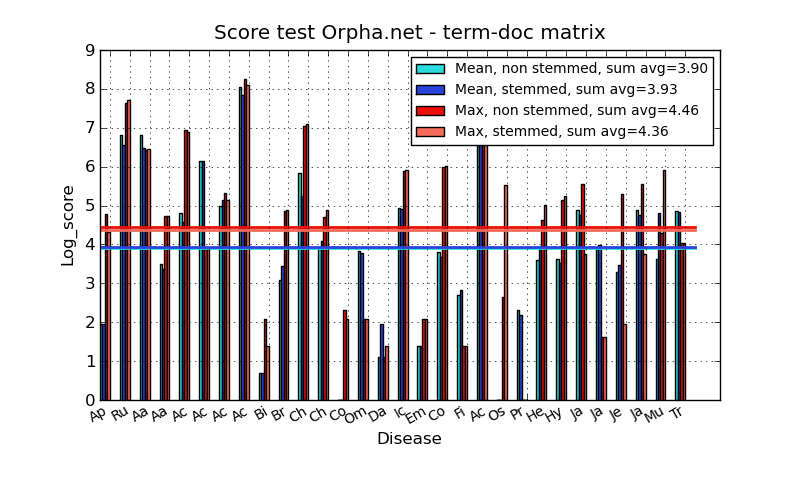
\includegraphics[width=1.2\textwidth]{barcharts/termDoc_orphan_hist_3000_ns_s_mea_max_sum.png}
  \end{center}
  \label{termDoc_orphan_hist_3000_ns_s_mea_max_sum}
\end{figure} 

\begin{table}[H]
\label{testResult_termDoc_orphan_hist_3000_ns_s_mea_max_sum}
\begin{tiny}
  \begin{tabular}{|l|r|r|r|r|r|r|r|r|r|r|r|r|r|r|r|r|r|r|r|r|r|r|r|r|r|r|r|r|r|r|r|}
    \hline
    Measure &Ap&Ru&Aa&Aa&Ac&Ac&Ac&Ac&Bi&Br&Ch&Ch&Co&Om&Da\\
    \hline
    Sum: mean non-stemmed &6&910&917&32&122&460&145&3119&1&21&342&50&0&45&2\\
    \hline
    Sum: mean stemmed &6&708&644&28&97&460&170&2522&1&30&190&58&0&43&6\\
    \hline
    Sum: max non-stemmed &119&2081&611&113&1031&48&203&3833&7&127&1139&109&9&7&2\\
    \hline
    Sum: max stemmed &75&2228&638&113&993&48&171&3281&3&131&1194&131&7&7&3 \\
    \hline
    \multicolumn{16}{c}{} \\
    \end{tabular}
    \begin{tabular}{|l|r|r|r|r|r|r|r|r|r|r|r|r|r|r|r|r|r|r|r|r|r|r|r|r|r|r|r|r|r|r|}
    \hline
     Measure &Ic&Em&Co&Fi&Ac&Os&Pr&He&Hy&Ja&Ja&Je&Ja&Mu&Tr &\scriptsize{\textbf{\# in top 20}} \\
    \hline
    Sum: mean non-stemmed &137&3&44&14&2458&0&9&36&37&132&47&26&132&37&127 & \scriptsize{\textbf{8}} \\
    \hline
    Sum: mean stemmed &136&3&39&16&2636&0&8&50&33&115&53&31&115&121&124 & \scriptsize{\textbf{8}} \\
    \hline
    Sum: max non-stemmed &357&7&401&3&1957&13&0&102&169&260&4&198&260&72&55 & \scriptsize{\textbf{9}} \\
    \hline
    Sum: max stemmed &365&7&414&3&2242&253&0&150&188&42&4&6&42&372&55 & \scriptsize{\textbf{9}} \\
    \hline
  \end{tabular}
\end{tiny}
\end{table}

We see here that the 'mean sum' similarity measure clearly outperforms the 'max sum'. 
In section \ref{DiseaseMatrix}, we compare this measure with the best of the cosine 
measure on and the term document and disease matrices.

\subsection{Disease and term document matrix - cosine, and sum and final result}

Now that we have found the results for the best measures to be used on
the term document matrix, we focus our attention on the disease
matrix. We will in the following test the sum and cosine measure
on the disease matrix and --- in the end of the section --- compare these
results to that of the term document matrix.

In the first test, we look at the performance of the cosine (mean),
cosine-sqrt and the sum measure on the BMJ and Orpha.net test
sets. These test are performed on both the non-stemmed and
stemmed. The results are shown on the figures
\ref{diseaseMatrix_bmj_hist_norm_3000_ns_cos_sqrt_cos_sum_nn},
\ref{diseaseMatrix_orphan_hist_NOTnorm_3000_ns_cos_sqrt_cos_sum_nn},
\ref{diseaseMatrix_bmj_hist_norm_3000_s_cos_sqrt_cos_sum_nn} and
\ref{diseaseMatrix_orphan_hist_NOTnorm_3000_s_cos_sqrt_cos_sum_nn}
below:

\textbf{Non-stemmed:}

\begin{figure}[H]
  \caption{Test of cosine measure (with and without sqrt-transformation) and sum measure on a non-stemmed disease matrix}
  \begin{center}
    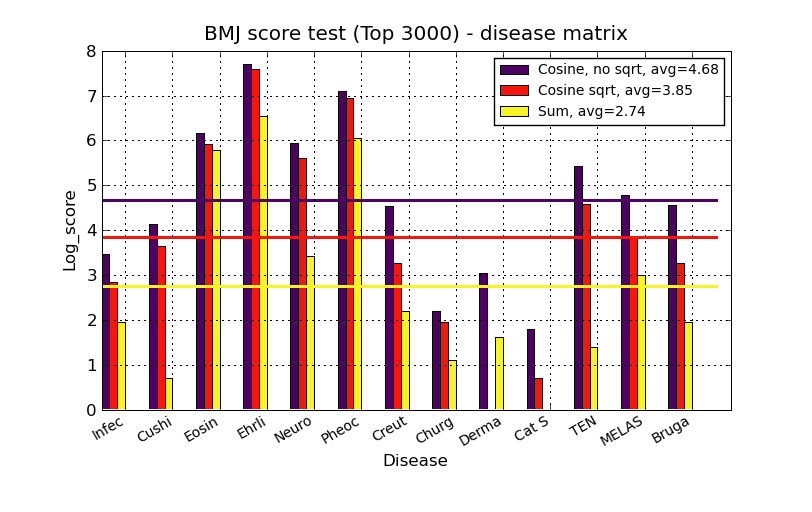
\includegraphics[width=1.2\textwidth]{barcharts/diseaseMatrix_bmj_hist_norm_3000_ns_cos_sqrt_cos_sum_nn.png}
  \end{center}
  \label{diseaseMatrix_bmj_hist_norm_3000_ns_cos_sqrt_cos_sum_nn}
\end{figure}

\begin{table}[H]
  \begin{tiny}
    \label{testResult_diseaseMatrix_bmj_hist_norm_3000_ns_cos_sqrt_cos_sum_nn}
    \begin{tabular}{|l|r|r|r|r|r|r|r|}
      \hline
      Measure &Infec&Cushi&Eosin&Ehrli&Neuro&Pheoc&Creut \\
      \hline
      Cosine no sqrt non-stemmed &31&62&474&2220&377&1225&93 \\
      \hline
      Cosine sqrt non-stemmed &16&37&375&2001&270&1037&25 \\
      \hline
      Sum non-stemmed &6&1&323&691&30&427&8  \\
      \hline
      \multicolumn{8}{c}{} \\
    \end{tabular}
    \begin{tabular}{|l|r|r|r|r|r|r|r|}
      \hline
      Measure &Churg&Derma&Cat S&TEN&MELAS&Bruga& \scriptsize{\textbf{\# in top 20}} \\
      \hline
      Cosine no sqrt non-stemmed &8&20&5&227&118&94 &\scriptsize{\textbf{2}} \\
      \hline
      Cosine sqrt non-stemmed &6&0&1&97&45&25 &  \scriptsize{\textbf{4}}\\
      \hline
      Sum non-stemmed &2&4&0&3&19&6 & \scriptsize{\textbf{9}} \\
      \hline
    \end{tabular}
  \end{tiny}
\end{table}

\begin{figure}[H]
  \caption{Test of cosine measure (with and without sqrt-transformation) and sum measure on a non-stemmed disease matrix}
  \begin{center}
    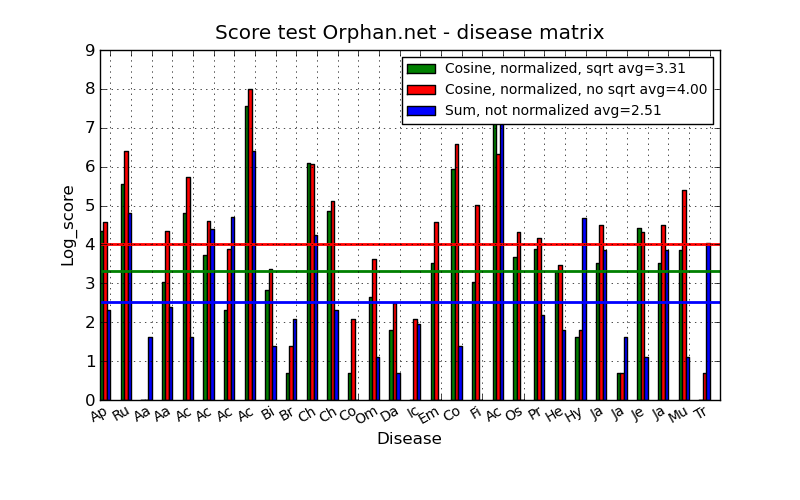
\includegraphics[width=1.2\textwidth]{barcharts/diseaseMatrix_orphan_hist_NOTnorm_3000_ns_cos_sqrt_cos_sum_nn.png}
  \end{center}
  \label{diseaseMatrix_orphan_hist_NOTnorm_3000_ns_cos_sqrt_cos_sum_nn}
\end{figure}

\begin{table}[H]
  \label{testResult_diseaseMatrix_orphan_hist_NOTnorm_3000_ns_cos_sqrt_cos_sum_nn}
  \begin{tiny}
    \begin{tabular}{|l|r|r|r|r|r|r|r|r|r|r|r|r|r|r|r|r|r|r|r|r|r|r|r|r|r|r|r|r|r|r|r|}
      \hline
      Measure &Ap&Ru&Aa&Aa&Ac&Ac&Ac&Ac&Bi&Br&Ch&Ch&Co&Om&Da\\
      \hline
      Cosine no sqrt non-stemmed &95&599&0&76&307&99&47&2989&28&3&430&165&7&37&11 \\
      \hline
      Cosine sqrt non-stemmed &76&257&0&20&122&41&9&1912&16&1&448&128&1&13&5 \\
      \hline
      Sum non-stemmed &9&123&4&10&4&81&109&601&3&7&68&9&0&2&1\\
      \hline
      \multicolumn{16}{c}{} \\
    \end{tabular}
    \begin{tabular}{|l|r|r|r|r|r|r|r|r|r|r|r|r|r|r|r|r|r|r|r|r|r|r|r|r|r|r|r|r|r|r|}
      \hline
      Measure &Ic&Em&Co&Fi&Ac&Os&Pr&He&Hy&Ja&Ja&Je&Ja&Mu&Tr &  \scriptsize{\textbf{\# in top 20}} \\
      \hline
      Cosine no sqrt non-stemmed &7&97&717&150&562&74&64&31&5&89&1&75&89&222&1 & \scriptsize{\textbf{8}} \\
      \hline
      Cosine sqrt non-stemmed &0&33&380&20&1687&39&47&26&4&33&1&83&33&46&0 &\scriptsize{\textbf{11}} \\
      \hline
      Sum non-stemmed &6&0&3&0&3000&0&8&5&107&46&4&2&46&2&55 & \scriptsize{\textbf{20}} \\
      \hline
    \end{tabular}
  \end{tiny}
\end{table}

\textbf{Stemmed:}

\begin{figure}[H]
  \caption{Test of cosine measure (with and without sqrt-transformation) and sum measure on a stemmed disease matrix}
  \begin{center}
    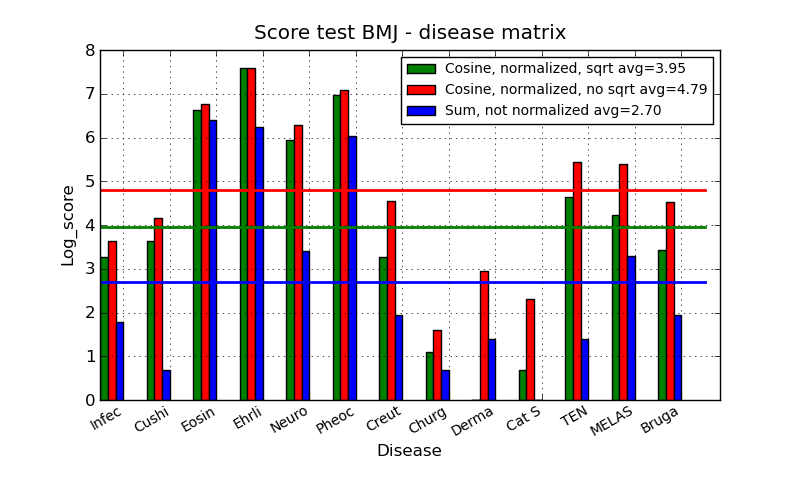
\includegraphics[width=1.2\textwidth]{barcharts/diseaseMatrix_bmj_hist_norm_3000_s_cos_sqrt_cos_sum_nn.png}
  \end{center}
  \label{diseaseMatrix_bmj_hist_norm_3000_s_cos_sqrt_cos_sum_nn}
\end{figure}

\begin{table}[H]
  \begin{tiny}
    \label{testResult_diseaseMatrix_bmj_hist_norm_3000_s_cos_sqrt_cos_sum_nn}
    \begin{tabular}{|l|r|r|r|r|r|r|r|}
      \hline
      Measure &Infec&Cushi&Eosin&Ehrli&Neuro&Pheoc&Creut \\
      \hline
      Cosine no sqrt stemmed &37&63&872&1963&533&1198&93 \\
      \hline
      Cosine sqrt stemmed &25&37&748&1970&384&1053&25 \\
      \hline
      Sum stemmed &5&1&597&511&29&413&6 \\
      \hline
      \multicolumn{8}{c}{} \\
    \end{tabular}
    \begin{tabular}{|l|r|r|r|r|r|r|r|}
      \hline
      Measure &Churg&Derma&Cat S&TEN&MELAS&Bruga& \scriptsize{\textbf{\# in top 20}} \\
      \hline
      Cosine no sqrt stemmed &4&18&9&230&221&91 &\scriptsize{\textbf{3}} \\
      \hline
      Cosine sqrt stemmed &2&0&1&102&68&30 &  \scriptsize{\textbf{3}}\\
      \hline
      Sum stemmed &1&3&0&3&26&6 & \scriptsize{\textbf{8}} \\
      \hline
    \end{tabular}
  \end{tiny}
\end{table}

\begin{figure}[H]
  \caption{Test of cosine measure (with and without sqrt-transformation) and sum measure on a stemmed disease matrix}
  \begin{center}
    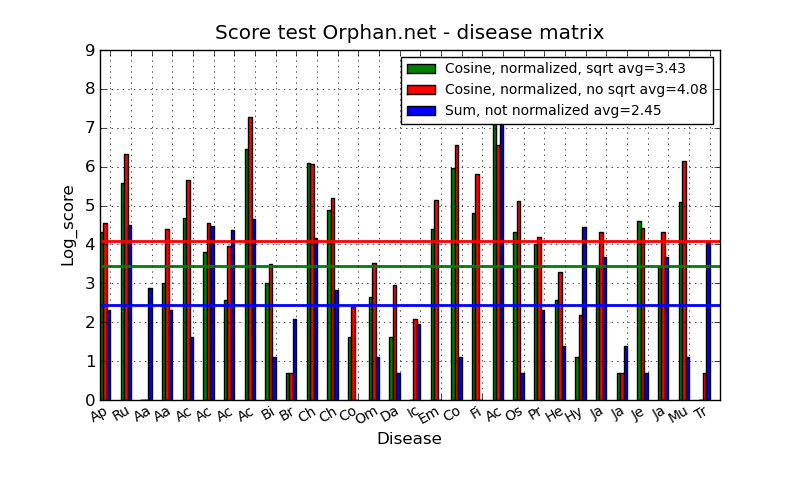
\includegraphics[width=1.2\textwidth]{barcharts/diseaseMatrix_orphan_hist_NOTnorm_3000_s_cos_sqrt_cos_sum_nn.png}
  \end{center}
  \label{diseaseMatrix_orphan_hist_NOTnorm_3000_s_cos_sqrt_cos_sum_nn}
\end{figure}

\begin{table}[H]
  \label{testResult_diseaseMatrix_orphan_hist_NOTnorm_3000_s_cos_sqrt_cos_sum_nn}
  \begin{tiny}
    \begin{tabular}{|l|r|r|r|r|r|r|r|r|r|r|r|r|r|r|r|r|r|r|r|r|r|r|r|r|r|r|r|r|r|r|r|}
      \hline
      Measure &Ap&Ru&Aa&Aa&Ac&Ac&Ac&Ac&Bi&Br&Ch&Ch&Co&Om&Da\\
      \hline
      Cosine no sqrt stemmed &94&553&0&80&284&94&51&1454&32&1&433&181&10&33&18 \\
      \hline
      Cosine sqrt stemmed &74&263&0&19&106&44&12&635&19&1&446&133&4&13&4 \\
      \hline
      Sum stemmed &9&90&17&9&4&86&79&105&2&7&64&16&0&2&1\\
      \hline
      \multicolumn{16}{c}{} \\
    \end{tabular}
    \begin{tabular}{|l|r|r|r|r|r|r|r|r|r|r|r|r|r|r|r|r|r|r|r|r|r|r|r|r|r|r|r|r|r|r|}
      \hline
      Measure &Ic&Em&Co&Fi&Ac&Os&Pr&He&Hy&Ja&Ja&Je&Ja&Mu&Tr &  \scriptsize{\textbf{\# in top 20}} \\
      \hline
      Cosine no sqrt stemmed &7&169&710&334&704&167&65&26&8&74&1&83&74&468&1 & \scriptsize{\textbf{8}} \\
      \hline
      Cosine sqrt stemmed &0&80&391&122&2137&74&54&12&2&30&1&99&30&162&0 &\scriptsize{\textbf{13}} \\
      \hline
      Sum stemmed &6&0&2&0&3000&1&9&3&84&39&3&1&39&2&59 & \scriptsize{\textbf{20}} \\
      \hline
    \end{tabular}
  \end{tiny}
\end{table}

When it comes to scoring diseases on in the disease matrix, the sum measure greatly out rival the 
cosine measure - with or without the square root transformation. If we look at the average values 
of the returned results, it seems that the stemmed version of the disease matrix is the best choice 
for optimized performance.

For the final test of measure and model, we compare the top results of the two matrices - term 
document and disease matrix. We will compare the different scores from the stemmed version of 
both matrix types since this seems to provide the overall best performance. In the figures 
\ref{termDoc_bmj_hist_3000_sum_dm_mea_cos_sqrt_td_max_cos_sqrt_td_mea_sum_td} and 
\ref{termDoc_orphan_hist_3000_sum_dm_mea_cos_sqrt_td_max_cos_sqrt_td_mea_sum_nn_td} below are 
bar chart of the best scores found for the prototype system:

\begin{figure}[H]
  \caption{Comparison of the mean sum measure, and mean and max sqrt cosine measure, on a stemmed term-doc matrix, and of the sum measure on a stemmed disease matrix}
  \begin{center}
    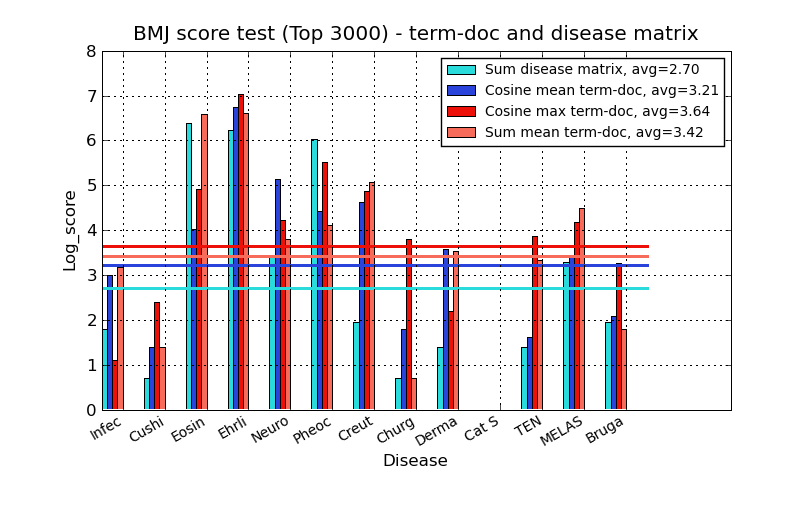
\includegraphics[width=1.2\textwidth]{barcharts/termDoc_bmj_hist_3000_sum_dm_mea_cos_sqrt_td_max_cos_sqrt_td_mea_sum_td.png}
  \end{center}
  \label{termDoc_bmj_hist_3000_sum_dm_mea_cos_sqrt_td_max_cos_sqrt_td_mea_sum_td}
\end{figure}

\begin{table}[H]
  \begin{tiny}
    \label{testResult_termDoc_bmj_hist_3000_sum_dm_mea_cos_sqrt_td_max_cos_sqrt_td_mea_sum_td}
    \begin{tabular}{|l|r|r|r|r|r|r|r|}
      \hline
      Measure &Infec&Cushi&Eosin&Ehrli&Neuro&Pheoc&Creut \\
      \hline
      Sum: disease matrix &5&1&597&511&29&413&6 \\
      \hline
      Cosine: term-doc mean-sqrt &19&3&22&1268&115&105&108 \\
      \hline
      Cosine: term-doc max-sqrt &2&10&136&1123&68&249&130 \\
      \hline
      Sum: term-doc mean &23&3&720&746&44&60&158 \\
      \hline
      \multicolumn{8}{c}{} \\
    \end{tabular}
    \begin{tabular}{|l|r|r|r|r|r|r|r|}
      \hline
      Measure &Churg&Derma&Cat S&TEN&MELAS&Bruga& \scriptsize{\textbf{\# in top 20}} \\
      \hline
      Sum: disease matrix &1&3&0&3&26&6 &\scriptsize{\textbf{8}} \\
      \hline
      Cosine: term-doc mean-sqrt &5&54&0&2&41&7 &\scriptsize{\textbf{6}}\\
      \hline
      Cosine: term-doc max-qrt &44&8&0&47&65&25 & \scriptsize{\textbf{4}} \\
      \hline
      Sum: term-doc mean &1&33&0&27&88&5 & \scriptsize{\textbf{4}} \\
      \hline
    \end{tabular}
  \end{tiny}
\end{table}

\begin{figure}[H]
  \caption{Comparison of the mean sum measure, and mean and max sqrt cosine measure, on a stemmed term-doc matrix, and of the sum measure on a stemmed disease matrix}
  \begin{center}
    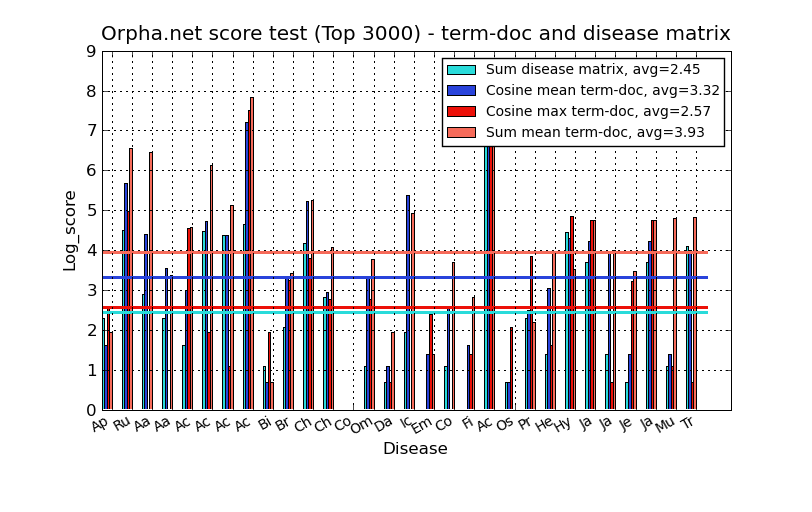
\includegraphics[width=1.2\textwidth]{barcharts/termDoc_orphan_hist_3000_sum_dm_mea_cos_sqrt_td_max_cos_sqrt_td_mea_sum_nn_td.png}
  \end{center}
  \label{termDoc_orphan_hist_3000_sum_dm_mea_cos_sqrt_td_max_cos_sqrt_td_mea_sum_nn_td}
\end{figure}

\begin{table}[H]
\label{testResult_termDoc_orphan_hist_3000_sum_dm_mea_cos_sqrt_td_max_cos_sqrt_td_mea_sum_nn_td}
\begin{tiny}
  \begin{tabular}{|l|r|r|r|r|r|r|r|r|r|r|r|r|r|r|r|r|r|r|r|r|r|r|r|r|r|r|r|r|r|r|r|}
    \hline
    Measure &Ap&Ru&Aa&Aa&Ac&Ac&Ac&Ac&Bi&Br&Ch&Ch&Co&Om&Da\\
    \hline
    Sum: disease matrix &9&90&17&9&4&86&79&105&2&7&64&16&0&2&1\\
    \hline
    Cosine: term-doc mean-sqrt &4&725&75&37&38&85&68&1651&1&23&80&15&0&26&2\\
    \hline
    Cosine: term-doc max-sqrt &12&145&0&0&93&6&2&1842&6&25&44&15&0&15&1\\
    \hline
    Sum: term-doc mean &6&708&644&28&97&460&170&2522&1&30&190&58&0&43&6 \\
    \hline
    \multicolumn{16}{c}{} \\
    \end{tabular}
    \begin{tabular}{|l|r|r|r|r|r|r|r|r|r|r|r|r|r|r|r|r|r|r|r|r|r|r|r|r|r|r|r|r|r|r|}
    \hline
     Measure &Ic&Em&Co&Fi&Ac&Os&Pr&He&Hy&Ja&Ja&Je&Ja&Mu&Tr &\scriptsize{\textbf{\# in top 20}} \\
    \hline
    Sum: disease matrix &6&0&2&0&3000&1&9&3&84&39&3&1&39&2&59 & \scriptsize{\textbf{20}} \\
    \hline
    Cosine: term-doc mean-sqrt &218&3&13&2&3000&1&9&14&78&84&48&3&84&1&62 & \scriptsize{\textbf{13}} \\
    \hline
    Cosine: term-doc max-sqrt &0&10&0&3&3000&7&46&4&128&115&1&24&115&2&1 & \scriptsize{\textbf{19}} \\
    \hline
    Sum: term-doc mean &136&3&39&16&2636&0&8&50&33&115&53&31&115&121&124 & \scriptsize{\textbf{8}} \\
    \hline
  \end{tabular}
\end{tiny}
\end{table}

Not only having the best average but also the right disease 9 out 13 (BMJ) and 20 out of 30 (Oprha.net) 
in the top 20 out of over 3000 diseases returned from a top 3000 document scores, using the simple sum 
similarity measure on a disease matrix seems to give both best recall and precision. This result is very 
interesting since the document-summed disease matrix was originally made as model for fast tests before 
implementation in the large term document matrix. This could imply that a summation of the document vectors 
for each individual disease seems to enhance the values of information carrying terms with the TF-IDF taking 
care of too common and non-information containing terms. The summation also efficiently eliminates the problem 
of noisy overview articles \ref{Overview}.

One of the noteworthy things that can be learned from the bar charts made in this and 
the two previous sections is that there should be a lower bound on the number of documents 
per disease. Acropectorovertebral dysplasia is a premium example that the system needs to 
have a lower bound on the number of MedLine records that are gathered for each disease. 
This is in order to ensure that the system will be able make a reasonable qualified guess 
on the disease.

\subsubsection{Clustering of the results}
\fxnote{Needs to be refined} 

We perform a clustering of the top 20 results using hierarchical
clustering. We have chosen to cluster the best disease from the sum
similarity measure on the stemmed disease matrix which is the
\textit{Cat Scratch disease}. Remember that the 20 diseases are chosen
based on the similarity to the query vector, not how similar they are
to each other. From figure
\ref{sum_stem_top20_best_cat_scratch_disease}, it can be seen that
\textit{Cat Scratch disease} (near the top) is clustered together with
\textit{Cyclic Neutropenia} even though it is number 19 on the result
list, this means these diseases are closest to each other in the list
of 20 returned suggestions. And the disease ranked as number 2 is
\textit{Kikuchi disease} which is 6 sub clusters away from \textit{Cat
  Scratch disease} - meaning that it requires merging 6 sub clusters
to get them into the same cluster, the merging is performed by
calculating a mean vector for the diseases (or sub clusters) being
merged. The lowest ranking disease is \textit{Chediak-Higashi
  syndrome}. To get this into the same cluster as \textit{Cat Scratch}
requires the merging of the entire cluster.

\begin{figure}[H]
  \begin{center}
    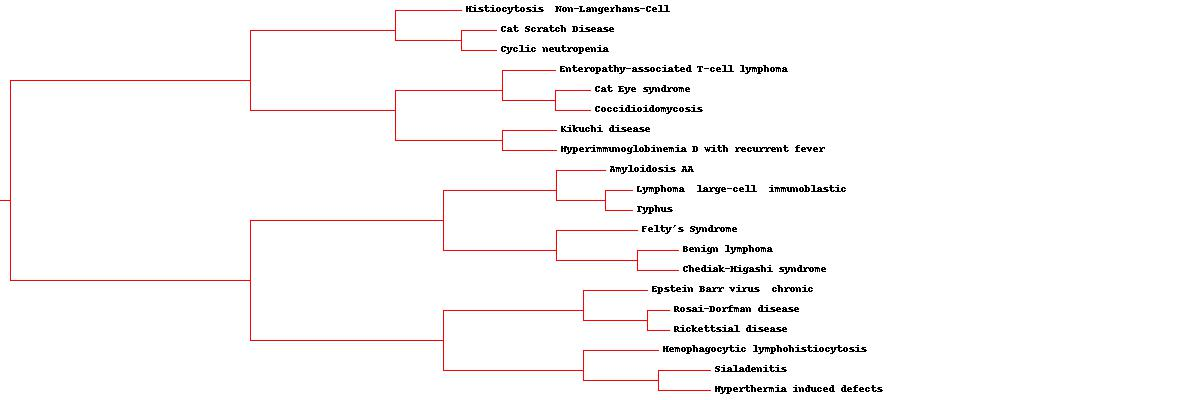
\includegraphics[width=1.3\textwidth]{clusters/sum_stem_top20_best_cat_scratch_disease.jpg}
  \end{center}
  \caption{Hierarchical clustering of best disease using sum, stemmed non-normalized}
  \label{sum_stem_top20_best_cat_scratch_disease}
\end{figure}

We have also chosen to cluster the disease where sum measure on the
stemmed disease matrix produced the worst result. This is the test
case \textit{Eosinophilic granuloma} where the correct disease was
ranked as number 597. Therefore it is not possible to find it in the
dendrogram. Our system suggested Developmental Dysplasia of Hip as
prime candidate given the query vector. Investigating the diseases
present in the dendrogram
\ref{sum_stem_top20_worst_developmental_dysplasia_of_hip} and
comparing them to the correct diagnosis of the disease (if found)
could provide helpful knowledge about why our system was so wrong in
its suggestion of this disease, and might provides clues to correcting
it. The problem might stem from bad or very noisy information about
the correct disease, which therefore do not provide enough similarity
to the query vector.

\begin{figure}[H]
  \begin{center}
    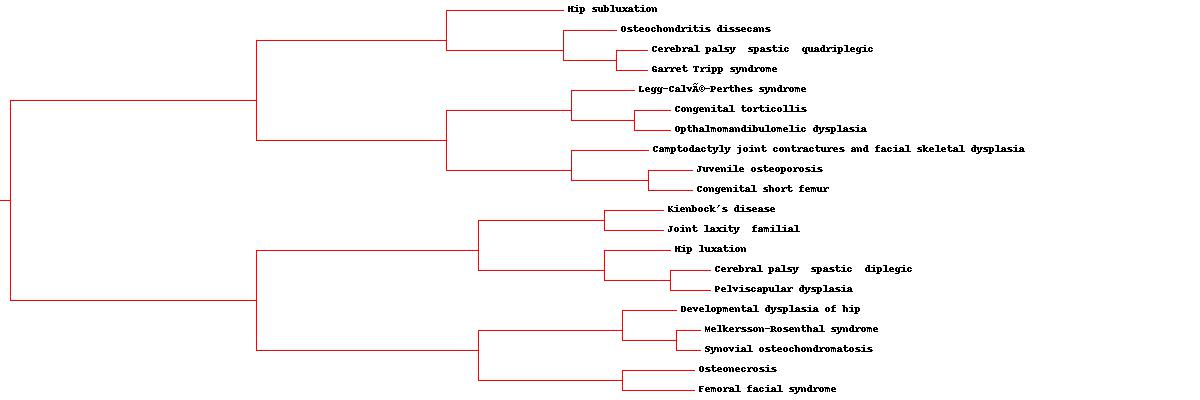
\includegraphics[width=1.3\textwidth]{clusters/sum_stem_top20_worst_developmental_dysplasia_of_hip.jpg}
  \end{center}
  \caption{Hierarchical clustering of worst disease using sum, stemmed non-normalized}
  \label{sum_stem_top20_worst_developmental_dysplasia_of_hip}
\end{figure}

\subsection{Results of the blind tests (provided by Henrik L. J\o rgensen)\label{Blindtest}}

Below are shown the results from from the blind tests described in table \ref{blind_test_table}.

\begin{figure}[H]
  \caption{Blind test of a stemmed disease matrix using the sum measure}
  \begin{center}
    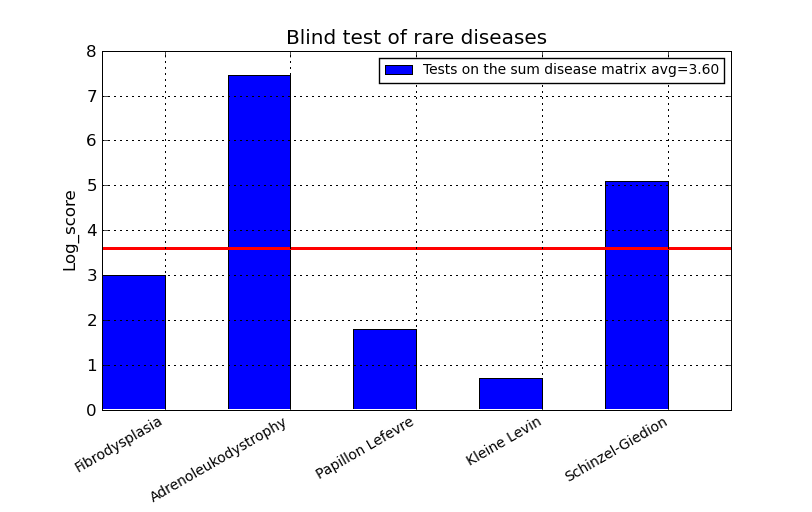
\includegraphics[width=1\textwidth]{barcharts/blind_test.png}
  \end{center}
  \label{blind_test_barchart}
\end{figure}

\begin{table}[H]
\begin{tiny}
  \begin{tabular}{|l|r|r|r|r|r|r|r|}
    \hline
    Measure & Fibrodysplasia & Adrenoleukodystrophy & Papillon Lefevre & Kleine Levin & Schinzel-Giedion & \scriptsize{\textbf{\# in top 20}}\\
    \hline
    Sum: disease matrix & 19 & 1717 & 5 & 1 & 164 & \scriptsize{\textbf{3}} \\
    \hline
    \end{tabular}
\end{tiny}
\end{table}

\noindent \small{\textit{*Note that the scores above are 0-indexed as in the previous sections.}}

\subsection{On overview article noise and consensus normalization\label{Overview}}

\subsubsection{Overview articles}
Unfortunately there is overview articles that can pollute the search
results and if overview articles are found in many of the top scoring
diseases, it could present a problem. When we run the consensus method
as described in section \ref{CosineScore}, an overview article would
potentially get an unfair high score since it gets summed up to 240
times. Though overview articles represents an element of noise, the
normalization of the vectors in the vector space model should in
theory down weight the highly summed documents. We also tested to the
most common overview article (240 occurrences) --- to see if it could
be a problem --- using the Orpha.net disease cases among top 3000
(documents). The overview article was present in less than 1 out of 8
searches which is not a significant amount. The disease matrix on the
other hand is less prone to the same problem, as it summarizes all
information about a disease into one vector.

\subsubsection{Consensus normalization}
During a point in the testing of the term document matrices, we got
the idea to try and divide each label with the number of documents it
had been summed over. This could in theory normalize the label in the
top score of returned results, as labels being over-represented in for
example the bottom of the top score list would be weighted down.
However, as this might be a good theoretical idea, it did not quite
amount to anything useful. The results for running this on the stemmed
term document matrix, using the cosine measures, is:\\

{\small
\noindent Mean: [99, 210, 804, 1216, 507, 667, 167, 309, 502, 50, 330, 695, 424] \\
Median: [1036, 989, 1432, 948, 668, 1301, 1315, 1687, 1429, 1233, 1696, 1494, 1322] \\
Max: [1034, 989, 1447, 1084, 635, 1284, 1293, 1687, 1414, 1233, 1696, 1491, 1321] \\
}

It does not take a bar chart to see that these values are pretty off
the top 20. The idea might be good enough but it would have to be on a
different model or data set than the one we use.
